\documentclass[12pt]{article}
\usepackage[margin=0.65in]{geometry} %to adjust page margins
%What is visible in tableofcontents? 
%0->part 1->section, 2->subsection, 3-> subsubsection 4->paragraph 5-> subparagraph
\setcounter{tocdepth}{4}
%To number until {No}
\setcounter{secnumdepth}{4}

%\usepackage{amsmath}
\usepackage[cm-default]{fontspec}
\setmainfont{Times New Roman}

%Greek hyphenation
\usepackage{xgreek}

\usepackage{graphicx}
\usepackage{listings}
%TO keep pictures and tables exactly where they are {H}
\usepackage{float}

\usepackage{caption}
\usepackage{mathtools}%text above arrows
%\usepackage{framed}
\usepackage{hyperref}%for links in refs
%\usepackage{placeins}%FloatBarrier (y)
\usepackage{fancyhdr}%page style
%\usepackage{color}

%About theorems, lemmas etc
\newtheorem{mydef}{Ορισμός}
\newtheorem{mylem}{Λήμμα}
\newtheorem{mytheorem}{Θεώρημα}
\newtheorem{theorem}{Theorem}[section]
\newtheorem{corollary}{Corollary}[theorem]
\newtheorem{lemma}[theorem]{Lemma}

%For algorithms
\usepackage[ruled,linesnumbered]{algorithm2e}

%For nice highlighting in code files
\usepackage[usenames,dvipsnames,svgnames,table]{xcolor}
\usepackage{color}
\definecolor{vimyellow}{rgb}{0.4,0.4,0}
\definecolor{vimblue}{rgb}{0,0,0.6}
\definecolor{mymauve}{rgb}{0.58,0,0.82}
\lstset{breaklines=true, xleftmargin=\parindent, language=C, keywordstyle=\color{vimyellow}, commentstyle=\color{vimblue},stringstyle=\color{red}, numbers=left, tabsize=3 }

%For reals set R, Q, 
\usepackage{amsfonts}

%\usepackage[•]{•}8x}{inputnc}

%2C "εικονα #" αντί για "Figure #"
\renewcommand{\figurename}{Εικόνα}
%2C "Πίνακας #" αντί για "Table #"
\renewcommand{\tablename}{Πίνακας}

%For more readable fractions
\newcommand\ddfrac[2]{\frac{\displaystyle #1}{\displaystyle #2}}

%Do not display date
\date{}
\pagestyle{fancy}
\lhead{Νευρωνικά Δίκτυα και Ευφυή Υπολογιστικά Συστήματα}
\rhead{Άσκηση 1}
%\pagenumbering{gobble}
\begin{document}
\begin{titlepage}
\date{}
\begin{center}

\includegraphics[width=0.2\textwidth]{logo_ntua.jpg}\\

\textsc{\LARGE Σχολη Ηλεκτρολογων Μηχανικων και Μηχανικων Υπολογιστων Ε.Μ.Π.}\\[1.5cm]
\LARGE
ΝΕΥΡΩΝΙΚΑ ΔΙΚΤΥΑ ΚΑΙ ΕΥΦΥΗ ΥΠΟΛΟΓΙΣΤΙΚΑ ΣΥΣΤΗΜΑΤΑ\\
2016-2017\\
\vfill
ΕΡΓΑΣΤΗΡΙΑΚΗ ΑΣΚΗΣΗ 2\\
\vfill
Ευαγγελία-Σοφία Γεργατσούλη\\
ΑΜ: 03112064\\
Νικηφόρος Μανδηλαράς\\
ΑΜ: 03112012\\
Εξάμηνο:9ο\\
\vfill
\end{center}
\end{titlepage}
%\tableofcontents %sections should me umbered to be included here
\newpage

\section*{Σκέλος 1ο - Υλοποίηση ενός SOM }
Πρώτο βήμα για την υλοποίηση της άσκησης ήταν η υλοποίηση τεσσάρων συναρτήσεων (somOutput.m, somActivation.m, somUpdate.m, somTrain.m) για την δημιουργία και εκπαίδευση ενός SOM.

\section*{Σκέλος 2ο - Μελέτη και ανάλυση SOM}
2Α. Σ' αυτό το σκέλος της άσκησης ζητήθηκε η κατασκευή χαρτών που εκπαιδεύονται βάσει δύο συνόλων δεδομένων. Επιλέξαμε μονοδιάστατα πλαίσια και για τα δύο σύνολα δεδομένων καθώς παρατηρήσαμε ότι ακολουθούν πολύ καλύτερα τη μορφή αυτών. Στη συνέχεια ακολουθούν τα αποτελέσματα για όλους τους συνδυασμούς τοπολογιών και αποστάσεων. Σε αυτή τη φάση για το   `οκτώ' χρησιμοποιήθηκαν 50 νευρώνες ενώ για το `ερωτηματικό' 20.

		\begin{figure}[H]
	 		\centering
			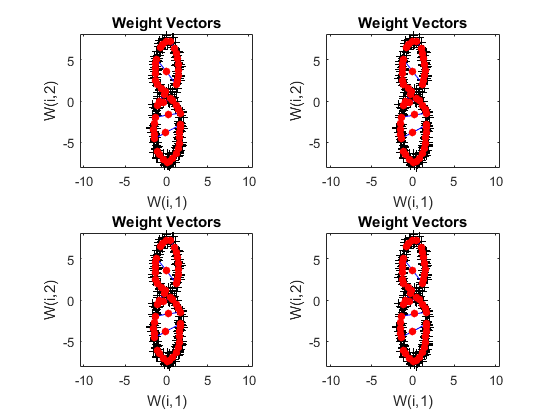
\includegraphics[width=0.8\textwidth]{fakelos/gridtop_eight.png}
			\caption{Εκτέλεση με τοπολογία gridtop για όλα τα μέτρα αποστάσεων με σειρά: boxdist,dist,linkdist,mandlist} 	  
			\label{fig:2}
		\end{figure} 
		\begin{figure}[H]
	 		\centering
			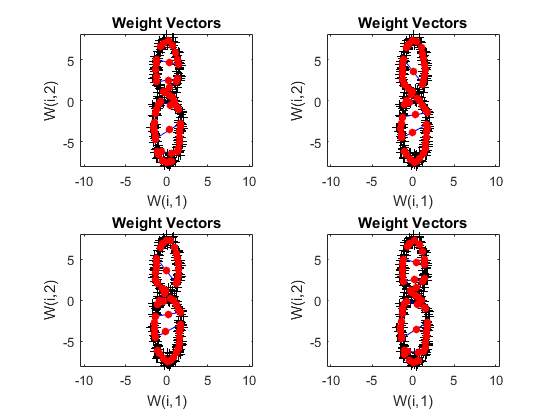
\includegraphics[width=0.8\textwidth]{fakelos/hextop_eight.png}
			\caption{Εκτέλεση με τοπολογία randtop για τις αποστάσεις ακολουθείται η ίδια σειρά με παραπάνω} 	  
			\label{fig:2}
		\end{figure} 		
		\begin{figure}[H]
	 		\centering
			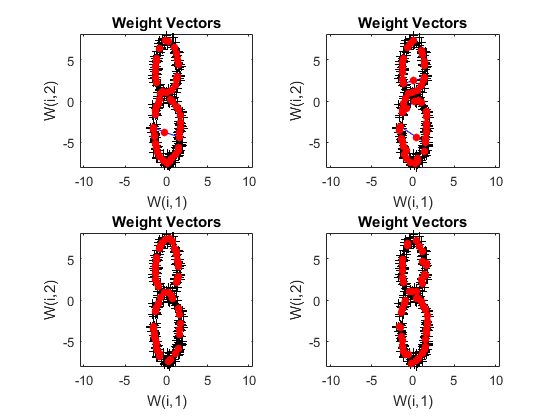
\includegraphics[width=0.8\textwidth]{fakelos/randtop_eight.png}
			\caption{Εκτέλεση με τοπολογία hextop} 	  
			\label{fig:2}
		\end{figure}
		\begin{figure}[H]
	 		\centering
			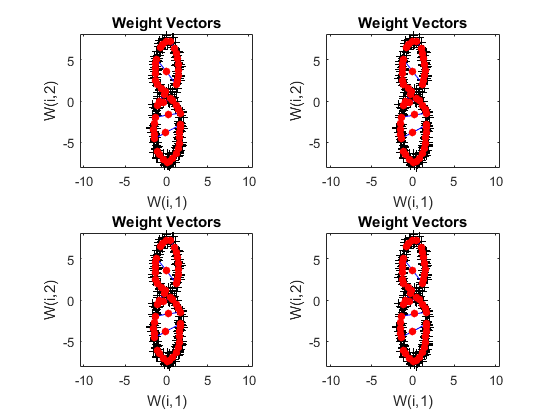
\includegraphics[width=0.8\textwidth]{fakelos/hexagonal_eight.png}
			\caption{Εκτέλεση με τοπολογία hexagonal} 	  
			\label{fig:2}
		\end{figure}
		
		\begin{figure}[H]
	 		\centering
			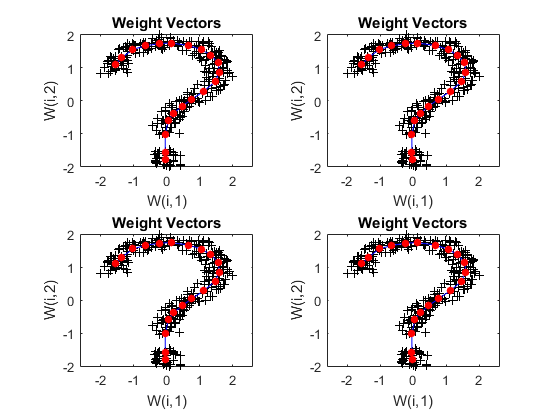
\includegraphics[width=0.8\textwidth]{fakelos/gridtop_question.png}
			\caption{Εκτέλεση με τοπολογία gridtop για όλα τα μέτρα αποστάσεων με σειρά: boxdist,dist,linkdist,mandlist} 	  
			\label{fig:2}
		\end{figure} 
		\begin{figure}[H]
	 		\centering
			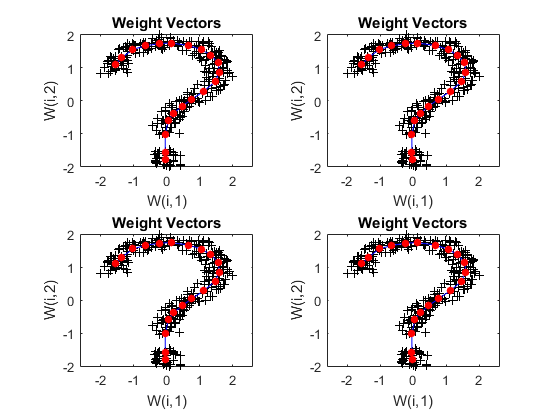
\includegraphics[width=0.8\textwidth]{fakelos/hextop_question.png}
			\caption{Εκτέλεση με τοπολογία randtop για τις αποστάσεις ακολουθείται η ίδια σειρά με παραπάνω} 	  
			\label{fig:2}
		\end{figure} 		
		\begin{figure}[H]
	 		\centering
			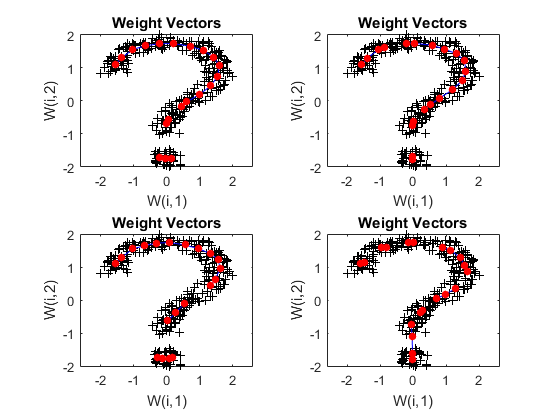
\includegraphics[width=0.8\textwidth]{fakelos/randtop_question.png}
			\caption{Εκτέλεση με τοπολογία hextop} 	  
			\label{fig:2}
		\end{figure}
		\begin{figure}[H]
	 		\centering
			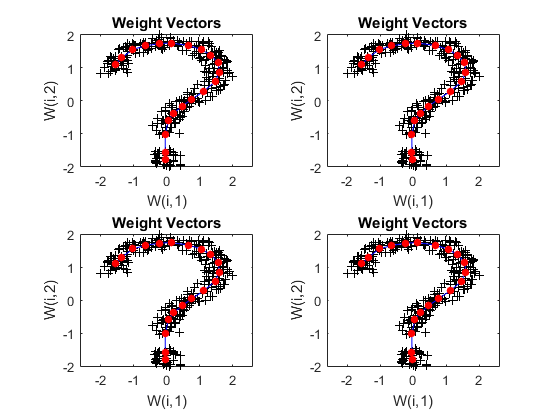
\includegraphics[width=0.8\textwidth]{fakelos/hexagonal_question.png}
			\caption{Εκτέλεση με τοπολογία hexagonal} 	  
			\label{fig:2}
		\end{figure}	
		
Παρατηρούμε ότι η επικάλυψη που υπάρχει για όλους τους συνδυασμούς τοπολογιών και αποστάσεων είναι πολύ καλή και για τα δύο σύνολα δεδομένων. Στη συνέχεια πειραματιζόμαστε ως προς το πλήθος των νευρώνων. Για το `ερωτηματικό' επιλέχθηκε το gridtop ως το τοπολογία και ως απόσταση το boxdist. Για το `οκτώ' το randtop και το linkdist. Πρώτα όμως παραθέτουμε τα αποτελέσματα για δισδιάστατο	πλαίσιο όπου φαίνεται ξεκάθαρα πως υστερούν σε σχέση με το μονοδιάστατο και έπειτα ακολουθούν οι παραστάσεις για μονοδιάστατο πλέγμα και διαφορετικούς αριθμούς νευρώνων.		
%		\begin{figure}[H]
%	 		\centering
%			\includegraphics[width=0.8\textwidth]{fakelos/.png}
%			\caption{} 	  
%			\label{fig:2}
%		\end{figure} 		 		 	
		\begin{figure}[H]
	 		\centering
			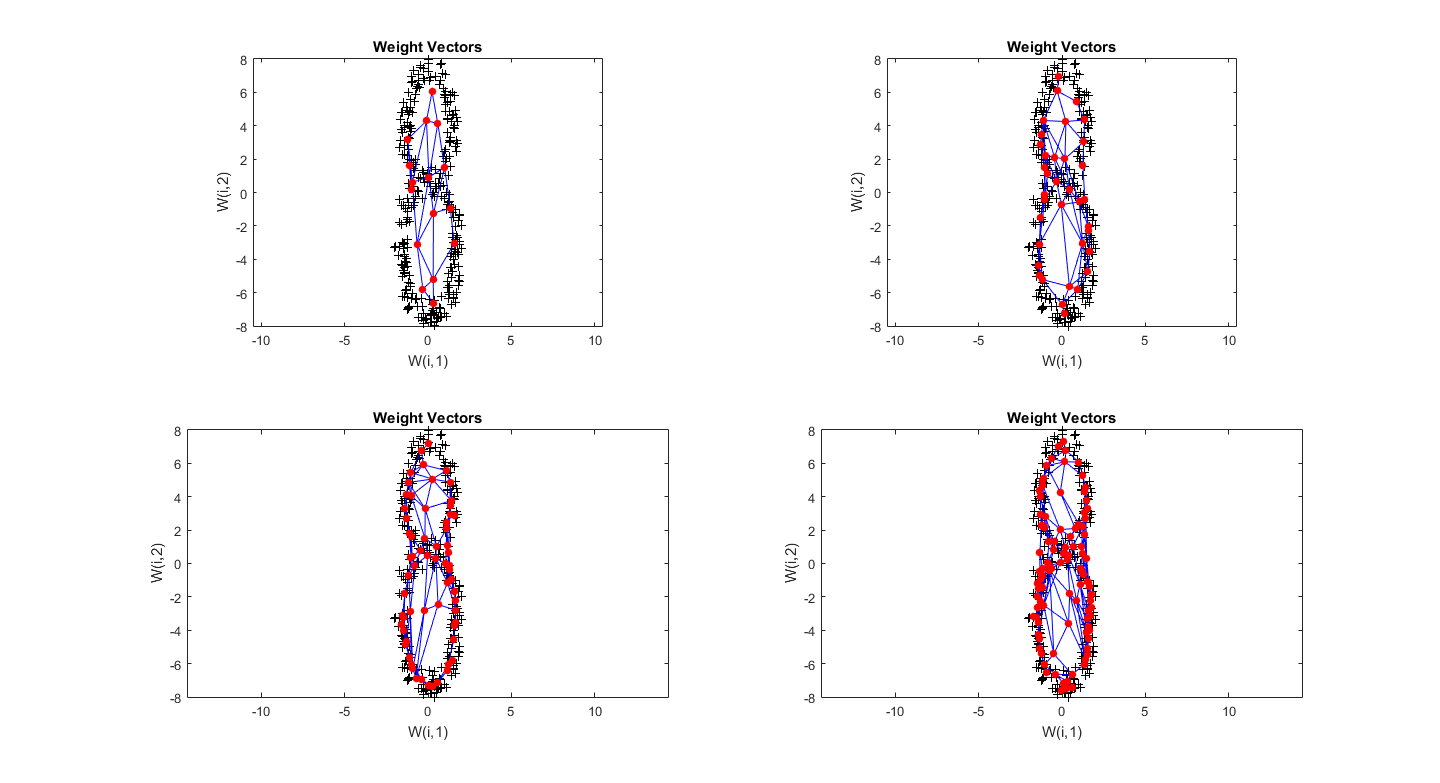
\includegraphics[width=0.8\textwidth]{fakelos/disdiastato_eight.png}
			\caption{Δισδιάστατο πλαίσιο με αριθμό νευρώνων ανά πλευρά 4,6,8,10} 	  
			\label{fig:2}
		\end{figure} 		
		\begin{figure}[H]
	 		\centering
			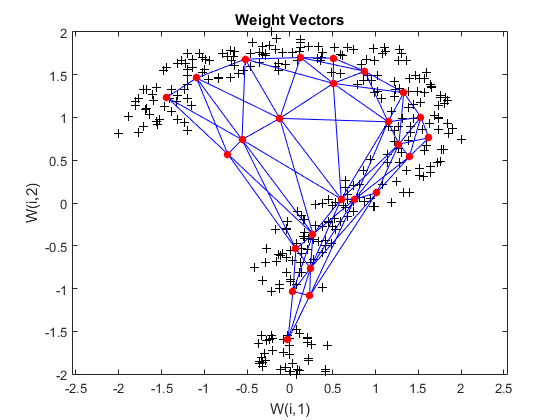
\includegraphics[width=0.8\textwidth]{fakelos/disdiastato_question.png}
			\caption{Δισδιάστατο πλαίσιο πλευράς 5} 	  
			\label{fig:2}
		\end{figure} 		
		\begin{figure}[H]
	 		\centering
			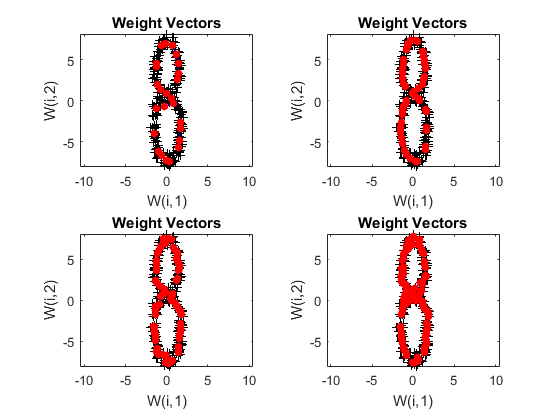
\includegraphics[width=0.8\textwidth]{fakelos/Eight_multinodes.png}
			\caption{Εκτέλεση για 25,50,75,100 νευρώνες} 	  
			\label{fig:2}
		\end{figure} 		 				
		\begin{figure}[H]
	 		\centering
			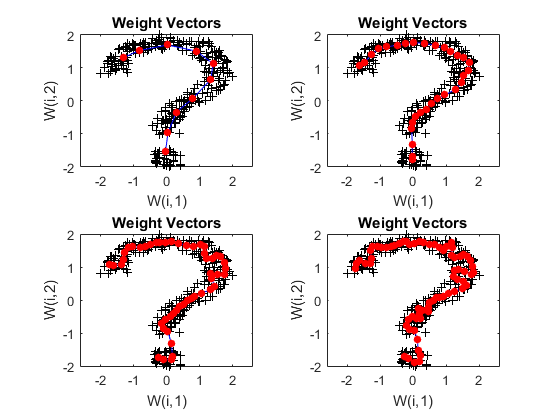
\includegraphics[width=0.8\textwidth]{fakelos/Question_multiplynodes.png}
			\caption{Εκτέλεση για 10,30,50,70 νευρώνες} 	  
			\label{fig:2}
		\end{figure} 		 			

Παρατητούμε ότι η αύξηση των νευρώνων στο πρώτο σύνολο επιδρά θετικά στην αποτύπωση του προτύπου ενώ στην περίπτωση του ερωτηματικού από τους 50 νευρώνες και έπειτα ο χάρτης αρχίζει να επικεντρώνεται στα μεμονωμένα σημεία της εισόδου.\\	

2B. Στη συνέχεια καλούμαστε να επιλήσουμε με τη χρήση ενός Som το πρόβλημα του περιοδεύοντος πωλητή. Γι αυτό το σκοπό χρησιμοποιήσαμε μονοδιάστατο πλέγμα με εξαγωνική τοπολογία και τη συνάρτηση ring distances για τον υπολογισμό των αποστάσεων. Όπως ήταν αναμενόμενο η προσέγγιση αυξανόταν σημαντικά με την αύξηση των νευρώνων. Πλήρη ταύτιση κόμβων με τις συνενταγμένες των πόλεων παρατηρούμε για αριθμό νευρώνων 80 παρόλο που οι πόλεις είναι μόλις 30.	
		\begin{figure}[H]
	 		\centering
			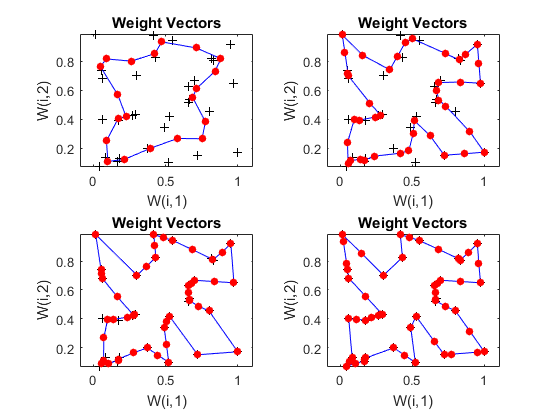
\includegraphics[width=0.8\textwidth]{fakelos/TSP.png}
			\caption{Πρόβλημα περιπλανώμενου πωλητή για 20,40,60,80 νευρώνες κατά σειρά} 	  
			\label{fig:2}
		\end{figure} 	
		
2Γ. 	Στο τρίτο αυτό μέρος ζητήθηκε η ομαδοποίηση ενός συνόλου δεδομένων, τα οποία συναποτελούσαν τον αριθμό `13'. Μετά την εκπαίδευση και δημιουργία του Som αποτυπώνουμε τον τρόπο με τον οποίο προσαρμόστηκαν οι νευρώνες σε έναν πίνακα ενοποιημένων αποστάσεων (U-matrix).  Στον πίνακα αυτό απεικονίζονται οι αποστάσεις του κάθε νευρώνα από τους γειτονικούς του. Έτσι λοιπόν για τους νευρώνες που ανήκουν στα σύνορα των δύο προτύπων είτε στο ενδιάμεσο οι αποστάσεις με τους γείτονες είναι μεγαλύτερες και συνεπώς το χρώμα αυτών στο U-matrix κινείται προς το κίτρινο. Για το συγκεκριμένο ερώτημα έγιναν τρείς εκτελέσεις, στην πρώτη χρησιμοποιήθηκε για τοπολογικό πλέγμα η randtop και ως τοπολογική γειτονιά η linkdist ενώ στη δεύτερη περίπτωση χρησιμοποιήθηκαν η hexagonalTopology και η linkdist ως πλέγμα και γειτονιά αντίστοιχα.Τέλος χρησιμοποιήθηκαν η gridtop και boxdist. Σε κάθε περίπτωση χρησιμοποιήσαμε χάρτη 10Χ10. H πρώτη ομάδα αποτελούσε τον `άσσο' του αριθμού σχηματίζεται από 144 πρότυπα ενώ το `τρία' από 206 σε σύνολο 350. Το πλήθος νευρώνων που ανατίθονται σε κάθε ομάδα διέφερε για την πρώτη εκτέλεση ο `άσσος' συγκέντρωσε 30 νευρώνες ενώ το `τρία' 70. Με τις παραμέτρους της δεύτερης εκτέλεσης είχαμε 66 νευρώνες για το ΄τρία΄ και 34 για τον `ἀσσο' ενώ και η τελευταία εκτέλεση είχε παράμοια νούμερα 63 και 34. Παρατηρούμε πως σε όλες τις περιπτώσεις η απόκλιση μεταξύ του πλήθους προτύπων κάθε ομάδας και του αντίστοιχου πλήθους νευρώνων είναι `υπέρ' του συνόλου που υπεραντιπροσωπεύται. Σ'αυτό το διαχωρισμό των νευρώνων δε λάβαμε υπόψιν μας όμως τους νευρώνες των συνόρων τους οποίους και κατατάξαμε στο κοντινότερο σύνολο. Παραθέτουμε παρακάτω τις απεικονίσεις του U-matrix αλλά και την οπτική αναπαράσταση του αποτελέσματος.
		\begin{figure}[H]
	 		\centering
			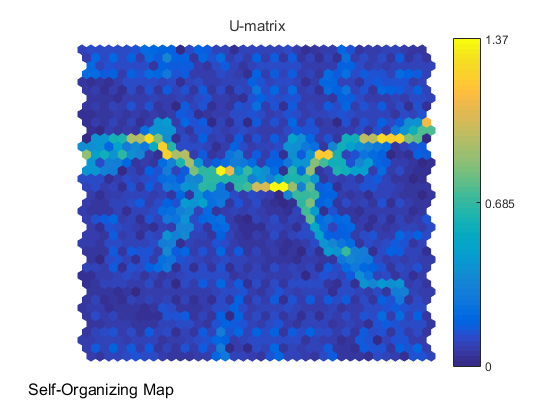
\includegraphics[width=0.8\textwidth]{fakelos/u-matrix.png}
			\caption{U-matrix για randtop και linkdist} 	  
			\label{fig:2}
		\end{figure} 		  
		\begin{figure}[H]
	 		\centering
			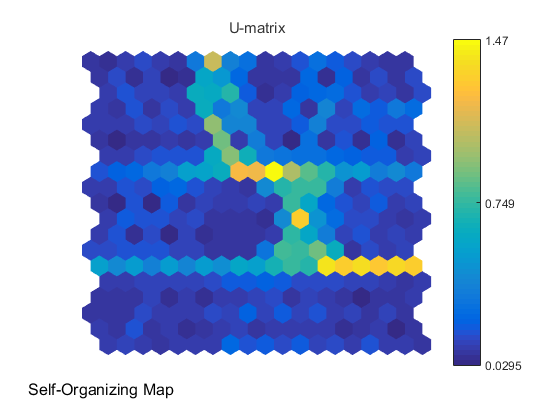
\includegraphics[width=0.8\textwidth]{fakelos/u-matrix2.png}
			\caption{} 	  
			\label{fig:2}
		\end{figure} 		 
		\begin{figure}[H]
	 		\centering
			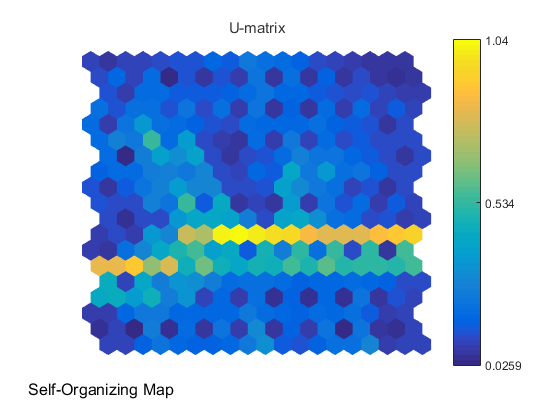
\includegraphics[width=0.8\textwidth]{fakelos/u-matrix11.png}
			\caption{} 	  
			\label{fig:2}
		\end{figure} 		
		\begin{figure}[H]
	 		\centering
			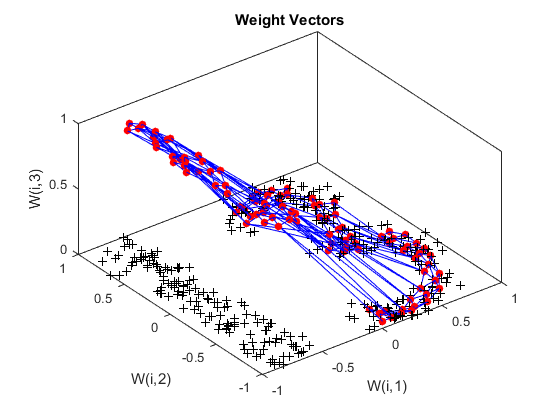
\includegraphics[width=0.8\textwidth]{fakelos/shapeof132.png}
			\caption{Ενδεικτική οπτική απεικόνιση} 	  
			\label{fig:2}
		\end{figure} 		   	
Από τα παραπάνω παρατηρούμε ότι η ομάδοποίηση που έχει γίνει είναι αρκετά καλή στην πρώτη και στην τρίτη περίπτωση, καθώς φαίνεται να σχηματίζονται τα πλαίσια των δύο συνόλων, ενώ στη δεύτερη υπάρχει απόκλιση από το αναμενόμενο. 		
\section*{Σκέλος 3ο - Document Clustering and Visualization }
				

%\section{Κώδικας}
%\subsection{Main}
%\label{subsec:main}
%\lstinputlisting[language=Matlab]{code/mainTotal.m}	
\end{document}
